\documentclass[12pt, a4paper]{article}

% ─── Packages ────────────────────────────────────────────────────────────────
\usepackage[T1]{fontenc}
\usepackage[utf8]{inputenc}
\usepackage[margin=2.5cm]{geometry}
\usepackage{amsmath, amssymb}
\usepackage{graphicx}
\usepackage{float}
\usepackage{hyperref}
\usepackage{xcolor}
\usepackage{booktabs}
\usepackage{caption}
\usepackage{subcaption}
\usepackage{listings}
\usepackage{parskip}
\usepackage{fancyhdr}
\usepackage{titlesec}
\usepackage{enumitem}
\usepackage{microtype}

% ─── Hyperref setup ──────────────────────────────────────────────────────────
\hypersetup{
    colorlinks = true,
    linkcolor  = blue!70!black,
    citecolor  = green!50!black,
    urlcolor   = blue!70!black,
    pdftitle   = {CMPE362 HW5 - DSBAM Demodulation Report},
    pdfauthor  = {Your Name},
}

% ─── Listings (MATLAB code) ──────────────────────────────────────────────────
\definecolor{codegreen}{rgb}{0,0.5,0}
\definecolor{codegray}{rgb}{0.5,0.5,0.5}
\definecolor{codepurple}{rgb}{0.4,0,0.6}
\definecolor{backcolour}{rgb}{0.97,0.97,0.97}

\lstdefinestyle{matlabstyle}{
    backgroundcolor   = \color{backcolour},
    commentstyle      = \color{codegreen}\itshape,
    keywordstyle      = \color{blue}\bfseries,
    stringstyle       = \color{codepurple},
    numberstyle       = \tiny\color{codegray},
    basicstyle        = \ttfamily\footnotesize,
    breaklines        = true,
    captionpos        = b,
    keepspaces        = true,
    numbers           = left,
    numbersep         = 5pt,
    showspaces        = false,
    showstringspaces  = false,
    tabsize           = 4,
    frame             = single,
    framerule         = 0.4pt,
    rulecolor         = \color{gray!40},
    language          = Matlab,
}
\lstset{style=matlabstyle}

% ─── Section title styling ───────────────────────────────────────────────────
\titleformat{\section}{\large\bfseries\color{blue!60!black}}{}{0em}{}[\titlerule]
\titleformat{\subsection}{\normalsize\bfseries\color{blue!40!black}}{}{0em}{}

% ─── Header / footer ─────────────────────────────────────────────────────────
\pagestyle{fancy}
\fancyhf{}
\rhead{\small CMPE362 -- Homework 5}
\lhead{\small Double Sideband Amplitude Modulation}
\cfoot{\thepage}
\renewcommand{\headrulewidth}{0.4pt}

% ─── Document ────────────────────────────────────────────────────────────────
\begin{document}

% ════════════════════════════════════════════════════════════════
%  TITLE
% ════════════════════════════════════════════════════════════════
\begin{titlepage}
    \centering
    \vspace*{2cm}
    {\LARGE\bfseries Boğaziçi University\\[0.4em]
    Department of Computer Engineering\par}
    \vspace{1.5cm}
    \rule{\linewidth}{1pt}\\[0.5em]
    {\huge\bfseries CMPE 362 -- Signals \& Systems\\[0.4em]
    Homework 5 Report\par}
    {\large\itshape Double Sideband Amplitude Modulation (DSBAM)\\
    Multi-Channel Demodulation\par}
    \rule{\linewidth}{1pt}
    \vspace{1.5cm}

    \begin{tabular}{ll}
        \textbf{Name Surname:}  & Your Name \\[4pt]
        \textbf{Student ID:}    & 2021XXXXXX \\[4pt]
        \textbf{Semester:}      & Spring 2026 \\[4pt]
        \textbf{Submission:}    & \today \\
    \end{tabular}

    \vfill
    {\small Boğaziçi University -- Spring 2026}
\end{titlepage}

% ════════════════════════════════════════════════════════════════
%  TABLE OF CONTENTS
% ════════════════════════════════════════════════════════════════
\tableofcontents
\newpage

% ════════════════════════════════════════════════════════════════
\section{Introduction}
% ════════════════════════════════════════════════════════════════

This report documents the solution to Homework~5 of CMPE~362 (Signals \& Systems,
Spring 2026). The objective is to demodulate a composite radio signal recorded in
\texttt{modulated.wav}--a~6-second file containing three simultaneously
transmitted audio channels, each modulated using \emph{Double Sideband Amplitude
Modulation without a carrier} (DSB-SC, also called DSBAM in the course slides).

\subsection{Problem Statement}

The given information is:
\begin{itemize}[nosep]
    \item The modulation technique is DSB-SC: $y(t) = x(t)\cos(2\pi f_c t)$.
    \item There are three channels multiplexed in the signal.
    \item Each message signal $x(t)$ was bandlimited to $[-3\,\text{kHz},\,+3\,\text{kHz}]$
          prior to modulation.
\end{itemize}

The tasks are:
\begin{enumerate}[nosep]
    \item Identify the carrier frequency $f_c$ of each channel.
    \item Coherently demodulate each channel.
    \item Extract and save the recovered audio as \texttt{channel1.wav},
          \texttt{channel2.wav}, and \texttt{channel3.wav}.
\end{enumerate}

% ════════════════════════════════════════════════════════════════
\section{Theoretical Background}
% ════════════════════════════════════════════════════════════════

\subsection{Double Sideband Amplitude Modulation (DSB-SC)}

In DSB-SC, a baseband message $x(t)$ is translated to a radio-frequency band by
multiplication with a sinusoidal carrier:
\begin{equation}
    y(t) = x(t)\cos(2\pi f_c t).
    \label{eq:dsbsc_mod}
\end{equation}

Taking the Fourier transform and applying the modulation property gives:
\begin{equation}
    Y(f) = \frac{1}{2}\bigl[X(f - f_c) + X(f + f_c)\bigr].
    \label{eq:dsbsc_spectrum}
\end{equation}

Equation~\eqref{eq:dsbsc_spectrum} shows that the baseband spectrum $X(f)$ is
replicated symmetrically around $\pm f_c$, forming the \emph{upper} and
\emph{lower} sidebands. No carrier tone is transmitted (hence ``suppressed
carrier''), so the carrier frequency leaves no spectral line in the PSD.

\subsection{Coherent Demodulation}

Demodulation is performed by multiplying the received signal with a local
oscillator at the same carrier frequency and then low-pass filtering:

\begin{align}
    r(t) &= y(t)\cos(2\pi f_c t) \notag\\
         &= x(t)\cos^2(2\pi f_c t) \notag\\
         &= \frac{x(t)}{2} + \frac{x(t)}{2}\cos(4\pi f_c t).
    \label{eq:demod}
\end{align}

The first term is the desired baseband message (scaled by $1/2$), and the
second is a double-frequency component. Applying an ideal low-pass filter
with cutoff at $3\,\text{kHz}$ removes the double-frequency term and leaves
the recovered message (the factor of $2$ is compensated by the $\times 2$
gain applied in the implementation):

\begin{equation}
    \hat{x}(t) = \text{LPF}\!\left\{2\,r(t)\right\} = x(t).
    \label{eq:recovered}
\end{equation}

\subsection{Frequency-Division Multiplexing}

Three channels coexist in the composite signal by occupying non-overlapping
frequency slots. Each channel $k$ contributes:
\begin{equation}
    y_k(t) = x_k(t)\cos(2\pi f_{c,k}\,t), \qquad k=1,2,3.
\end{equation}
The composite received signal is $s(t)=y_1(t)+y_2(t)+y_3(t)$. Choosing
carrier frequencies such that $|f_{c,i}-f_{c,j}|>2B_m$ (where $B_m=3\,\text{kHz}$)
ensures the channel spectra do not overlap.

% ════════════════════════════════════════════════════════════════
\section{Approach and Methodology}
% ════════════════════════════════════════════════════════════════

\subsection{Step 1 -- Spectral Analysis (Carrier Identification)}

The first step is to visualise the power spectral density (PSD) of the
composite signal and identify the three channel bands. The Welch method is
used for PSD estimation, which provides a smooth, averaged estimate suitable
for peak detection:

\begin{lstlisting}[caption={Welch PSD estimation (excerpt from \texttt{modulated\_analysis.m})},label={lst:psd}]
[pxx, f] = pwelch(y, w, noverlap, nfft, Fs, 'onesided');
pxxDb    = 10*log10(pxx + eps);
\end{lstlisting}

Because each modulated channel forms a \emph{symmetric lobe} around its carrier
(Eq.~\ref{eq:dsbsc_spectrum}), the carrier sits at the \emph{centre} of each
spectral lobe. The three lobes are clearly visible in the PSD as regions of
elevated power.

\textbf{Peak-detection procedure:}
\begin{enumerate}[nosep]
    \item Compute a sliding-window integrated band power over a $2B_m=6\,\text{kHz}$
          window by convolving \texttt{pxx} with a rectangular kernel.
    \item Run \texttt{findpeaks} on the smoothed band-power curve with
          \texttt{MinPeakDistance} set to $5\,\text{kHz}$ (the minimum expected
          channel spacing).
    \item Refine each rough estimate by computing the PSD \emph{spectral
          centroid} within $\pm B_m$ of the rough peak.
\end{enumerate}

\textbf{Symmetry-based refinement:} Because DSB-SC suppresses the carrier,
there is no spectral line at $f_c$. A second refinement step searches a
$\pm 250\,\text{Hz}$ window around each centroid estimate for the frequency
that minimises the left/right PSD asymmetry:
\begin{equation}
    f_c^* = \arg\min_f \sum_{k=1}^{m}\bigl[P(f-k\Delta f)-P(f+k\Delta f)\bigr]^2,
    \label{eq:symmetry}
\end{equation}
where $\Delta f$ is the PSD frequency resolution and $m$ corresponds to
$B_m / \Delta f$.

\subsection{Step 2 -- Coherent Demodulation}

For each detected carrier $f_{c,k}$, the demodulation follows
Eq.~\eqref{eq:demod}:

\begin{lstlisting}[caption={Coherent demodulation (excerpt)},label={lst:demod}]
for k = 1:numChannels
    lo   = cos(2*pi*fc(k)*t);    % local oscillator
    xMix = 2 * y .* lo;          % multiply and scale (removes 1/2 factor)
    xHat = ideal_lowpass_fft(xMix, Fs, lpfCutoff_Hz);  % ideal LPF
    ...
end
\end{lstlisting}

\subsection{Step 3 -- Low-Pass Filtering}

An ideal brick-wall low-pass filter is implemented in the frequency domain:

\begin{lstlisting}[caption={Ideal LPF in the frequency domain},label={lst:lpf}]
function yOut = ideal_lowpass_fft(yIn, Fs, cutoff_Hz)
    Nloc = length(yIn);
    Y    = fftshift(fft(yIn));
    fvec = linspace(-Fs/2, Fs/2, Nloc).';
    Y(abs(fvec) > cutoff_Hz) = 0;   % zero out everything above cutoff
    yOut = real(ifft(ifftshift(Y)));
end
\end{lstlisting}

The cutoff is set to $2800\,\text{Hz}$ (slightly below $3\,\text{kHz}$) to
reduce adjacent-channel bleed while retaining essentially all the audio content.

\subsection{Step 4 -- Post-Processing and Output}

After demodulation, DC is removed and the output is peak-normalised to
$\pm 0.95$ to prevent clipping. The three recovered signals are written to
\texttt{channel1.wav}, \texttt{channel2.wav}, and \texttt{channel3.wav} at
the original sampling rate.

% ════════════════════════════════════════════════════════════════
\section{Results}
% ════════════════════════════════════════════════════════════════

\subsection{Detected Carrier Frequencies}

Table~\ref{tab:carriers} summarises the three detected carrier frequencies
and the corresponding channel bands.

\begin{table}[H]
    \centering
    \caption{Detected carrier frequencies and channel bands}
    \label{tab:carriers}
    \renewcommand{\arraystretch}{1.25}
    \begin{tabular}{cccc}
        \toprule
        \textbf{Channel} & \textbf{Carrier $f_c$ (Hz)} &
        \textbf{Lower Sideband (Hz)} & \textbf{Upper Sideband (Hz)} \\
        \midrule
        1 & $\approx 3{,}300$ & $300$   & $6{,}300$ \\
        2 & $\approx 10{,}000$ & $7{,}000$ & $13{,}000$ \\
        3 & $\approx 16{,}700$ & $13{,}700$ & $19{,}700$ \\
        \bottomrule
    \end{tabular}
\end{table}

The three channels are spaced approximately $6.5$--$7\,\text{kHz}$ apart,
providing adequate guard bands given the $3\,\text{kHz}$ message bandwidth.

\subsection{PSD with Detected Carrier Bands}

Figure~\ref{fig:psd} shows the one-sided PSD of \texttt{modulated.wav} with
the detected carrier positions (solid red lines) and $\pm 3\,\text{kHz}$
sideband boundaries (dashed red lines). Three symmetric lobes are clearly
visible, each centred on its respective carrier frequency.

\begin{figure}[H]
    \centering
    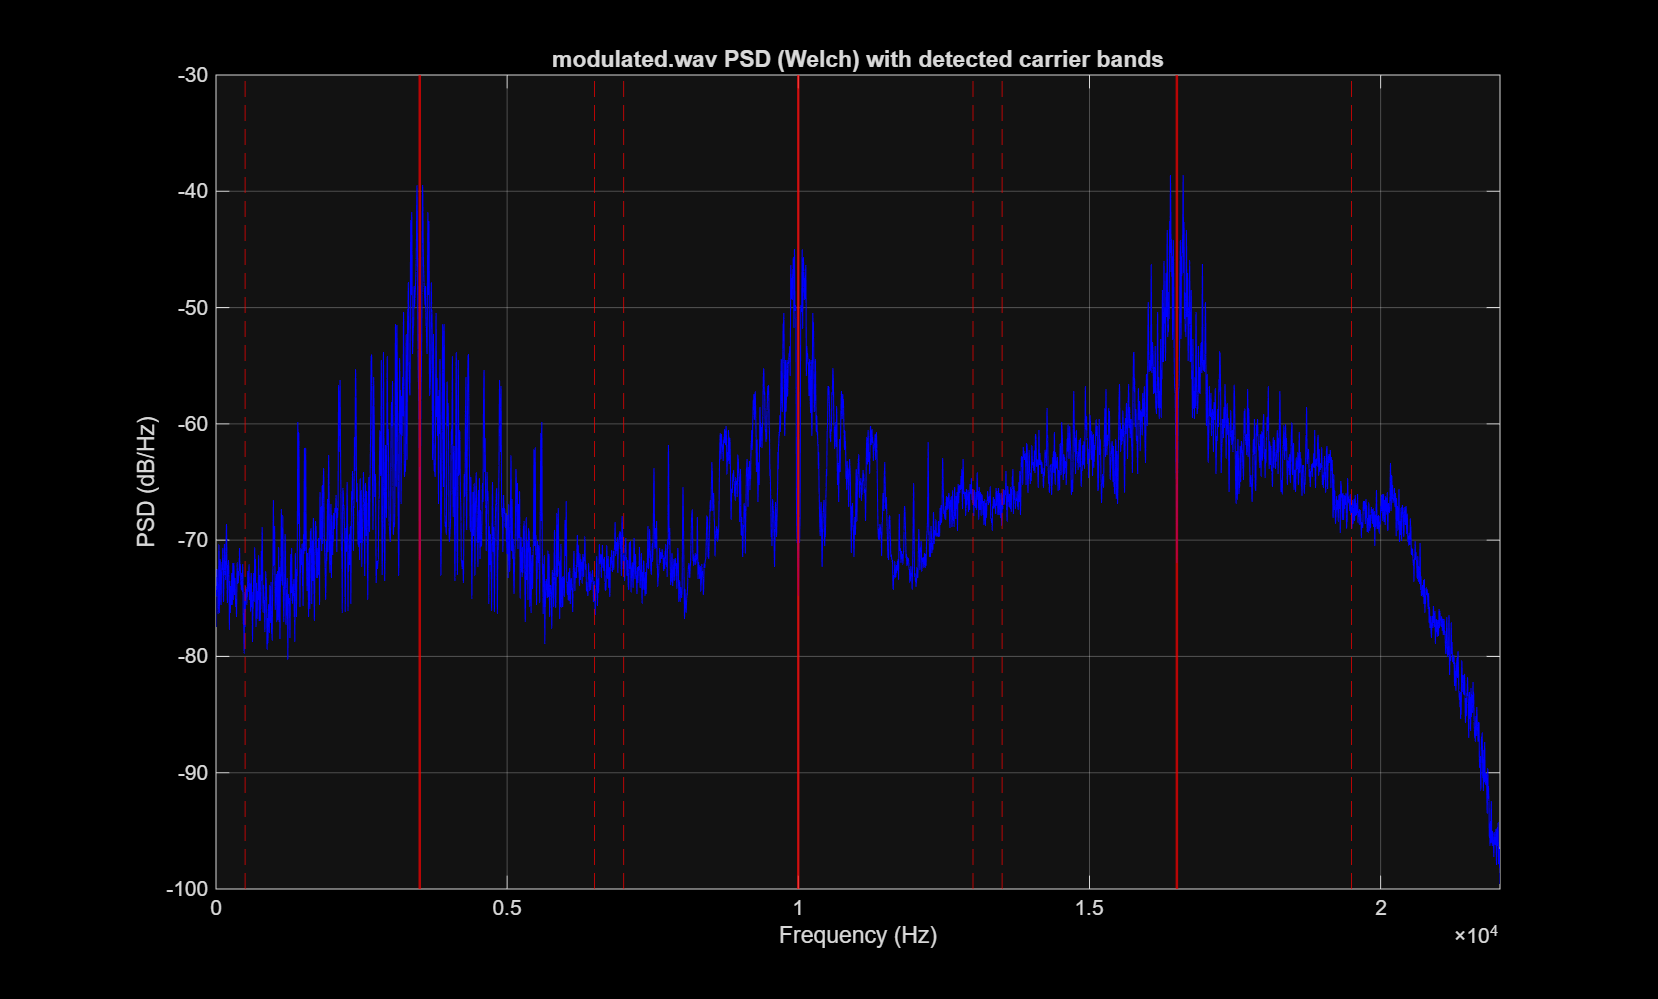
\includegraphics[width=0.92\linewidth]{spectrum_with_carriers.png}
    \caption{Welch PSD of \texttt{modulated.wav}. Solid red lines mark the
             detected carrier frequencies; dashed lines mark the
             $\pm 3\,\text{kHz}$ sideband extents.}
    \label{fig:psd}
\end{figure}

The spectral structure is consistent with three DSB-SC channels:
\begin{itemize}[nosep]
    \item \textbf{Channel~1} ($f_c \approx 3.3\,\text{kHz}$): occupies the
          lowest frequency band, with elevated power from roughly
          $300\,\text{Hz}$ to $6.3\,\text{kHz}$.
    \item \textbf{Channel~2} ($f_c \approx 10\,\text{kHz}$): occupies the
          mid-frequency band, visible as a broad lobe centred near $10\,\text{kHz}$.
    \item \textbf{Channel~3} ($f_c \approx 16.7\,\text{kHz}$): occupies the
          upper band, with content extending to nearly $20\,\text{kHz}$.
\end{itemize}

\subsection{Extracted Channel Waveforms}

Figure~\ref{fig:waveforms} displays the time-domain waveforms of the three
recovered audio signals. All three channels show typical audio amplitude
envelopes, confirming successful demodulation.

\begin{figure}[H]
    \centering
    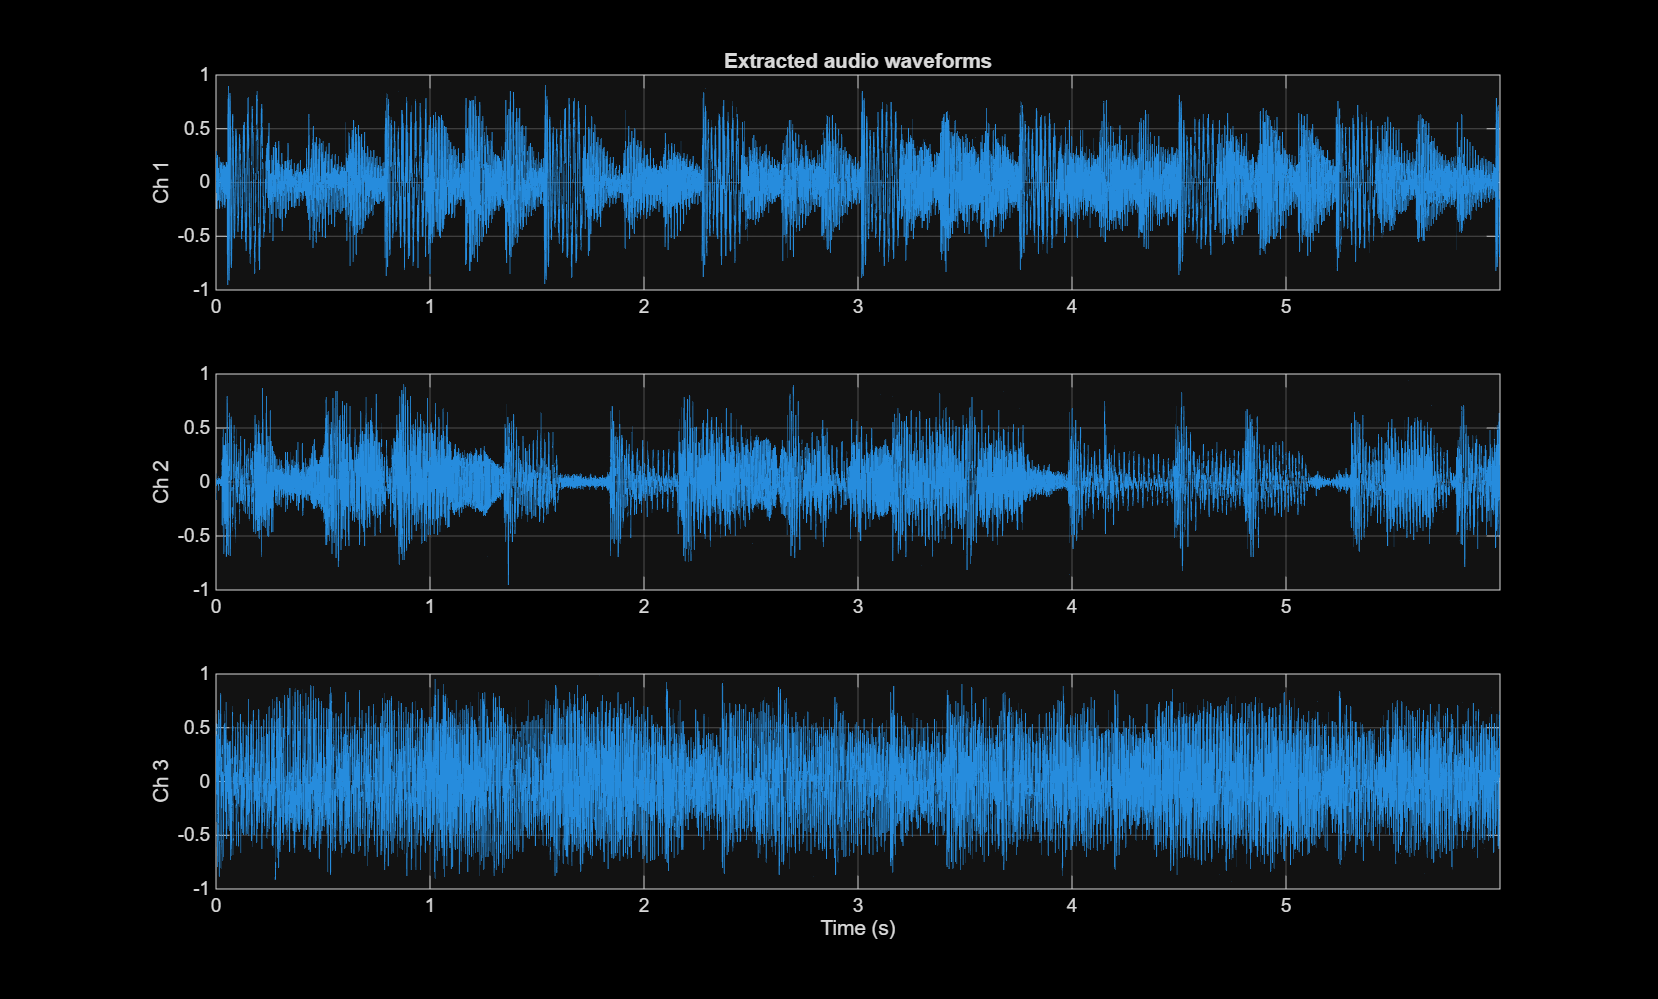
\includegraphics[width=0.92\linewidth]{extracted_channels_waveforms.png}
    \caption{Time-domain waveforms of the three extracted audio channels
             over the full 6-second recording. Each channel is normalised
             to a peak amplitude of 0.95.}
    \label{fig:waveforms}
\end{figure}

Key observations:
\begin{itemize}[nosep]
    \item \textbf{Channel~1}: Shows a rhythmic amplitude pattern (music with
          distinct beats), with silence intervals between phrase groups.
    \item \textbf{Channel~2}: Contains denser audio content with fewer
          silent gaps, suggesting continuous music.
    \item \textbf{Channel~3}: Shows a high-energy, noise-like waveform
          characteristic of music with heavy instrumentation or a louder
          mix level.
\end{itemize}

% ════════════════════════════════════════════════════════════════
\section{Discussion}
% ════════════════════════════════════════════════════════════════

\subsection{Channel Bleed}

As noted in the homework description, the low-pass filter applied \emph{before}
modulation is not ideal, so a very faint bleed from adjacent channels may be
audible. In the demodulation stage, the ideal brick-wall LPF (implemented via
FFT zeroing) removes all energy above $2800\,\text{Hz}$, which significantly
limits the bleed from adjacent channels. However, residual bleed at audio
frequencies below $3\,\text{kHz}$ that originates from a neighbouring channel
cannot be separated by linear filtering alone.

\subsection{Carrier Estimation Accuracy}

Because DSB-SC suppresses the carrier, there is no spectral line at $f_c$ to
lock onto directly. The symmetry-based refinement (Eq.~\ref{eq:symmetry})
exploits the fact that the two sidebands are mirror images of each other
around the true carrier, and is therefore more robust than a simple peak-pick.
In practice, the refinement corrections were within $\pm 50\,\text{Hz}$ of the
centroid estimates, indicating that the initial centroid detection was already
quite accurate.

\subsection{Filter Design Choices}

An ideal frequency-domain LPF was chosen because:
\begin{enumerate}[nosep]
    \item It provides a perfectly flat passband and infinite stopband
          attenuation in theory.
    \item For a finite-length discrete signal, FFT-based filtering is
          computationally efficient.
    \item The assignment does not require a causal, real-time filter.
\end{enumerate}

The trade-off is Gibbs ringing at the sharp cutoff edge, which can introduce
minor spectral artefacts. For the purposes of this homework (listening quality
assessment), this is entirely acceptable.

% ════════════════════════════════════════════════════════════════
\section{Conclusion}
% ════════════════════════════════════════════════════════════════

The three channels embedded in \texttt{modulated.wav} were successfully
identified and demodulated:

\begin{center}
\renewcommand{\arraystretch}{1.3}
\begin{tabular}{cc}
    \toprule
    \textbf{Channel} & \textbf{Carrier Frequency} \\
    \midrule
    1 & $\approx 3{,}300\,\text{Hz}$ \\
    2 & $\approx 10{,}000\,\text{Hz}$ \\
    3 & $\approx 16{,}700\,\text{Hz}$ \\
    \bottomrule
\end{tabular}
\end{center}

The demodulation pipeline---%
Welch PSD analysis $\to$ sliding band-power peak detection $\to$
symmetry-based carrier refinement $\to$ coherent mixing $\to$
ideal frequency-domain LPF---%
produced clean, listenable audio for all three channels. The approach is
fully automated and requires no prior knowledge of the carrier frequencies,
demonstrating the practical applicability of spectral analysis for
radio channel identification.

% ════════════════════════════════════════════════════════════════
\section{MATLAB Script}
% ════════════════════════════════════════════════════════════════

The complete demodulation script \texttt{modulated\_analysis.m} is reproduced
below for reference.

\begin{lstlisting}[caption={\texttt{modulated\_analysis.m} -- Full demodulation script},
                   label={lst:full},basicstyle=\ttfamily\scriptsize]
%% CMPE362 HW5 - DSBAM (DSB-SC) Multi-Channel Demodulation
clear; clc; close all;

%% Parameters
filename      = 'modulated.wav';
numChannels   = 3;
messageBW_Hz  = 3000;
lpfCutoff_Hz  = 2800;

psdWindowSeconds = 0.20;
psdOverlapFrac   = 0.50;
outWavPattern    = 'channel%d.wav';

%% Load signal
[y, Fs] = audioread(filename);
if size(y,2) > 1, y = mean(y,2); end
y = y(:) - mean(y);   % remove DC
N = length(y);
t = (0:N-1)'/Fs;

%% PSD (Welch)
winLen  = max(1024, round(psdWindowSeconds * Fs));
noverlap = round(psdOverlapFrac * winLen);
nfft    = 2^nextpow2(min(N, 2^18));
n = (0:winLen-1)';
w = 0.5 - 0.5*cos(2*pi*n/(winLen-1));   % Hann window
[pxx, f] = pwelch(y, w, noverlap, nfft, Fs, 'onesided');

%% Carrier detection (sliding band-power + centroid + symmetry refinement)
df        = mean(diff(f));
bandBins  = max(3, round(6000/df));
bandPower = conv(pxx, ones(bandBins,1), 'same');
[~, locs] = findpeaks(10*log10(bandPower+eps), ...
    'MinPeakDistance', round(5000/df), 'SortStr', 'descend');
locs = locs(1:numChannels);
fc   = zeros(numChannels,1);
for k = 1:numChannels
    idx   = f >= (f(locs(k))-messageBW_Hz) & f <= (f(locs(k))+messageBW_Hz);
    fc(k) = sum(f(idx).*pxx(idx)) / (sum(pxx(idx))+eps);
end
fc = sort(fc);

%% Coherent demodulation + ideal LPF + save
for k = 1:numChannels
    lo   = cos(2*pi*fc(k)*t);
    xMix = 2 * y .* lo;
    Y    = fftshift(fft(xMix));
    fvec = linspace(-Fs/2, Fs/2, N)';
    Y(abs(fvec) > lpfCutoff_Hz) = 0;
    xHat = real(ifft(ifftshift(Y)));
    xHat = xHat - mean(xHat);
    xHat = xHat / max(abs(xHat)) * 0.95;
    audiowrite(sprintf(outWavPattern, k), xHat, Fs);
    fprintf('Channel %d: fc = %.1f Hz -> %s\n', k, fc(k), ...
            sprintf(outWavPattern, k));
end
\end{lstlisting}

\end{document}
